\documentclass [xcolor=svgnames, t] {beamer} 
\usepackage[utf8]{inputenc}
\usepackage{booktabs, comment} 
\usepackage[absolute, overlay]{textpos} 
\usepackage{pgfpages}
\usepackage[font=footnotesize]{caption}
\useoutertheme{infolines} 
\usepackage{ragged2e}
\setbeamertemplate{caption}[numbered]
\definecolor{brownbrown}{RGB}{56, 28, 0}
\definecolor{brownred}{RGB}{228, 0, 43}

\setbeamercolor{title in head/foot}{bg=brownred, fg=brownbrown}
\setbeamercolor{author in head/foot}{bg=myuniversity}
\setbeamertemplate{page number in head/foot}{}
\usepackage{csquotes}

\usepackage{amsmath}
\usepackage[makeroom]{cancel}


\usepackage{textpos}

\usepackage{tikz}

\usetheme{Madrid}
\definecolor{myuniversity}{RGB}{56, 28, 0}
\usecolortheme[named=myuniversity]{structure}

\setbeamertemplate{bibliography item}[text]
\apptocmd{\thebibliography}{\justifying}{}{} 

\title[ARLU-Net]{Semantic Segmentation of Brain Tumor Images using Attention-based Residual Light U-Net Model}
%\subtitle{(Your Sub Title)}
\author[Chakrapani]{Chakrapani\\[4mm]{\small Supervisor: Dr. Sunil Kumar}}
\titlegraphic{
\includegraphics[height=2.0cm]{logo.pdf}}
\institute[2020IS-02]{ABV-IIITM, Gwalior}

\date{\today}


\addtobeamertemplate{navigation symbols}{}{%
    \usebeamerfont{footline}%
    \usebeamercolor[fg]{footline}%
    \hspace{1em}%
    \insertframenumber/\inserttotalframenumber
}

\begin{document}
\begin{frame}
\maketitle
\end{frame}


%%%%%%%%%%%%%%%%%%%%%%%%%%%%
%\logo{
\includegraphics[height=1.0cm]{logo.pdf}~%}
%%%%%%%%%%%%%%%%%%%%%%%%%%

\justifying

\begin{frame}
\frametitle{Table of Contents}
\tableofcontents
\end{frame}

\section{Introduction}
\begin{frame}\frametitle{Introduction brain tumor segmentation}
\begin{figure}[H]
\centering
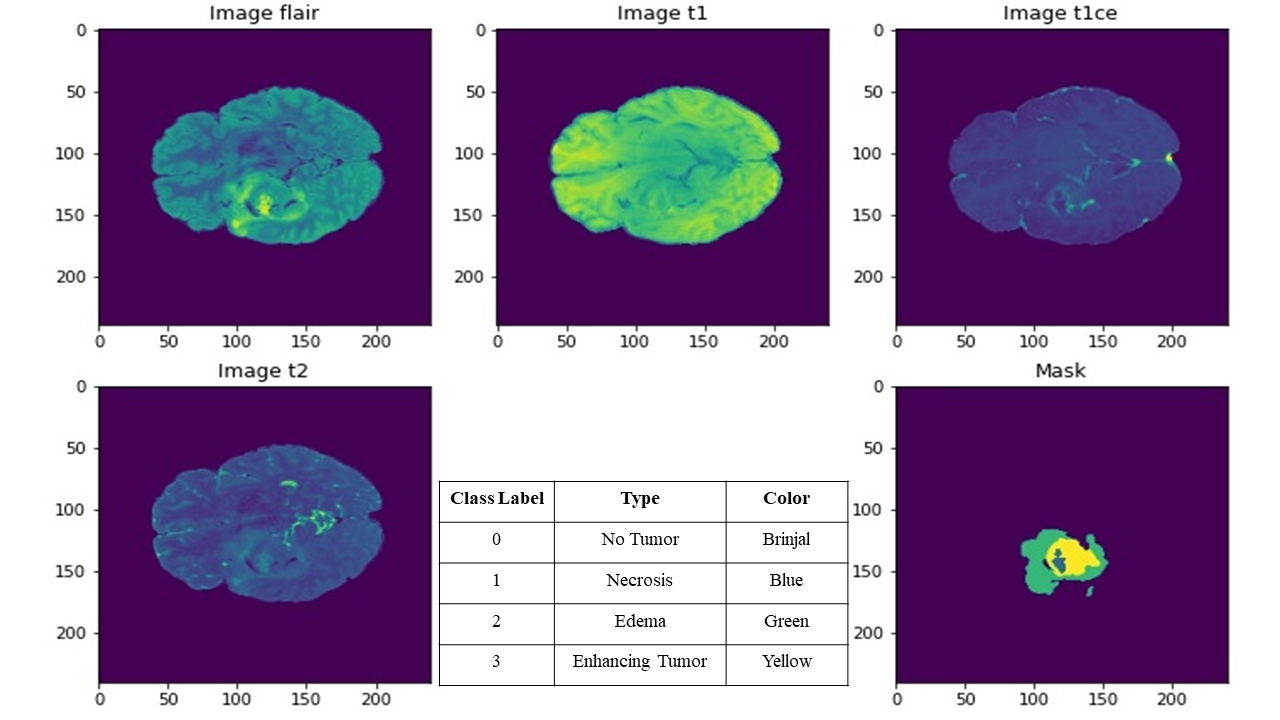
\includegraphics[width=12cm]{2021 sample.png}
\caption{Data sample of a patient with different axial view and ground truth image.}
\end{figure}
\end{frame}

\begin{frame}{Class imbalance problem}
    \begin{figure}[H]
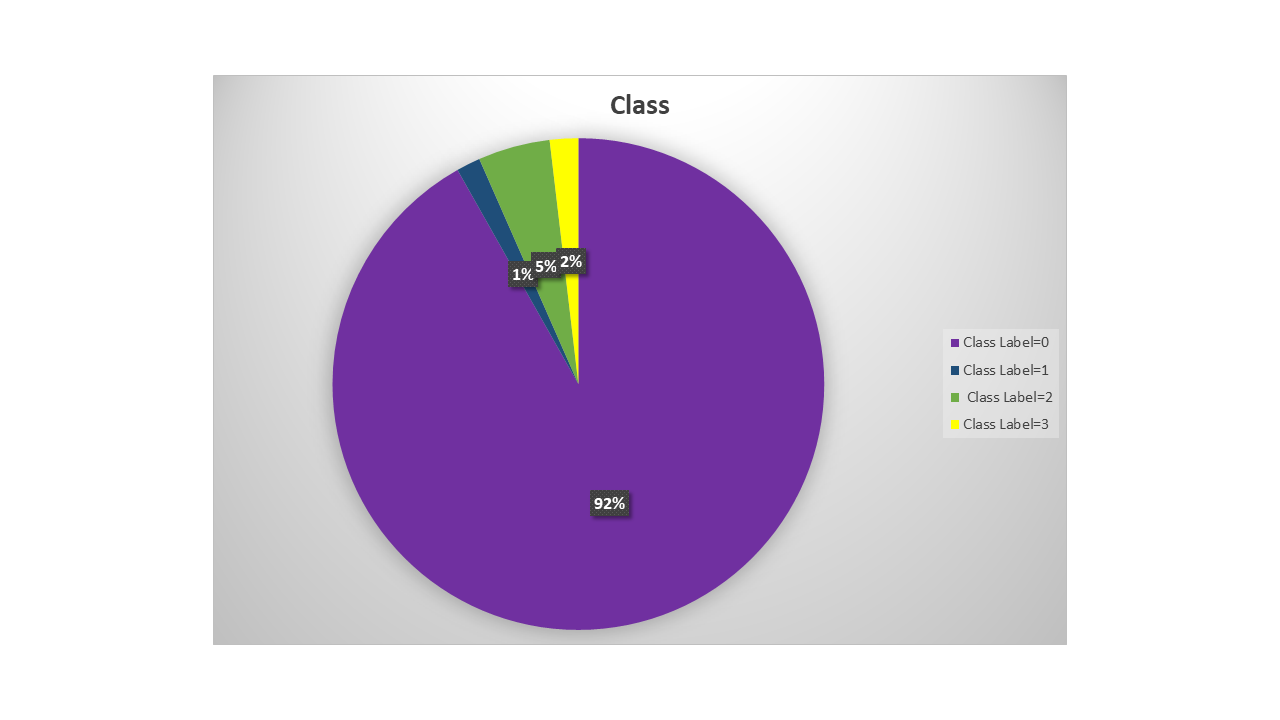
\includegraphics[width=1\linewidth]{class label.png}
\caption{Class labels with percent of pixel value in data samples}
\end{figure}
\end{frame}

\section{Objective}
\begin{frame}\frametitle{Objective}
\centering
\begin{center}
\vspace*{\fill}
\begin{enumerate}
\justifying
    \item To develop a method for segmenting brain tumor images.
    \item To explore the different state-of-art methods for brain tumor segmentation method.
    \item To come-up with the effecient light-weight model for brain tumor segmentation.
    \item To come-up with an efficient attention mechanism for brain tumor segmentation.
    \item To address class imbalance problem.
    \item To compare state-of-art method and proposed method for brain tumor segmentation problem.
\end{enumerate}
\vspace*{\fill}
\end{center}
\end{frame}

\section{Our contribution}
\begin{frame}{Our contribution}
\begin{center}
\vspace*{\fill}
\begin{enumerate}
\justifying
    \item We propose a light-weight ARLU-Net model for the brain tumor segmentation task. 
    \item The new attention mechanism is invoked to focus more on the tumor region, which is hard to segment. 
    \item We proposed a new loss function using weighted dice loss and weighted focal loss to handle the class imbalance problem.
    \item We validated our proposed model on the BraTS-2021 dataset, the latest publicly available dataset. We compared our model with state-of-art models, U-Net \cite{10.1007/978-3-319-24574-4_28}, ResU-Net \cite{SHEHAB2021404}, V-Net \cite{Milletari2016VNetFC} and ARU-Net \cite{MAJI2022103077}. 
\end{enumerate}

\vspace*{\fill}
\end{center}
\end{frame}

\section{Short comings in existing state-of-the-art}
\begin{frame}\frametitle{Short comings in existing state-of-the-art}
\begin{figure}[ht!]
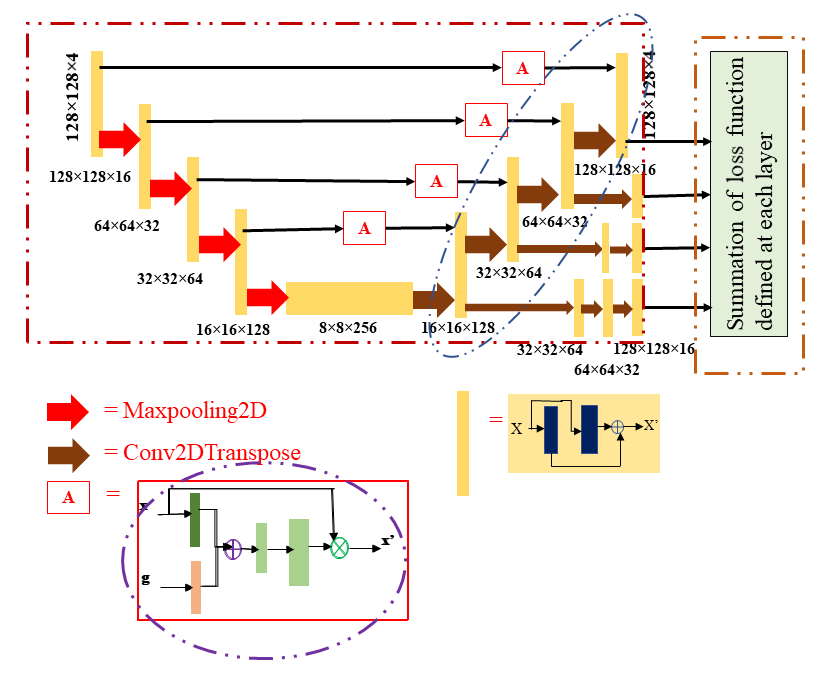
\includegraphics[width=0.7\linewidth]{baseline model.png}
\caption{Architecture of Attention based Residual U-Net\cite{MAJI2022103077}}
\centering
\end{figure}
\end{frame}

\section{Proposed ARLU-Net}
\begin{frame}{Proposed Attention-based Residual Light U-Net}
\begin{figure}[H]
\centering
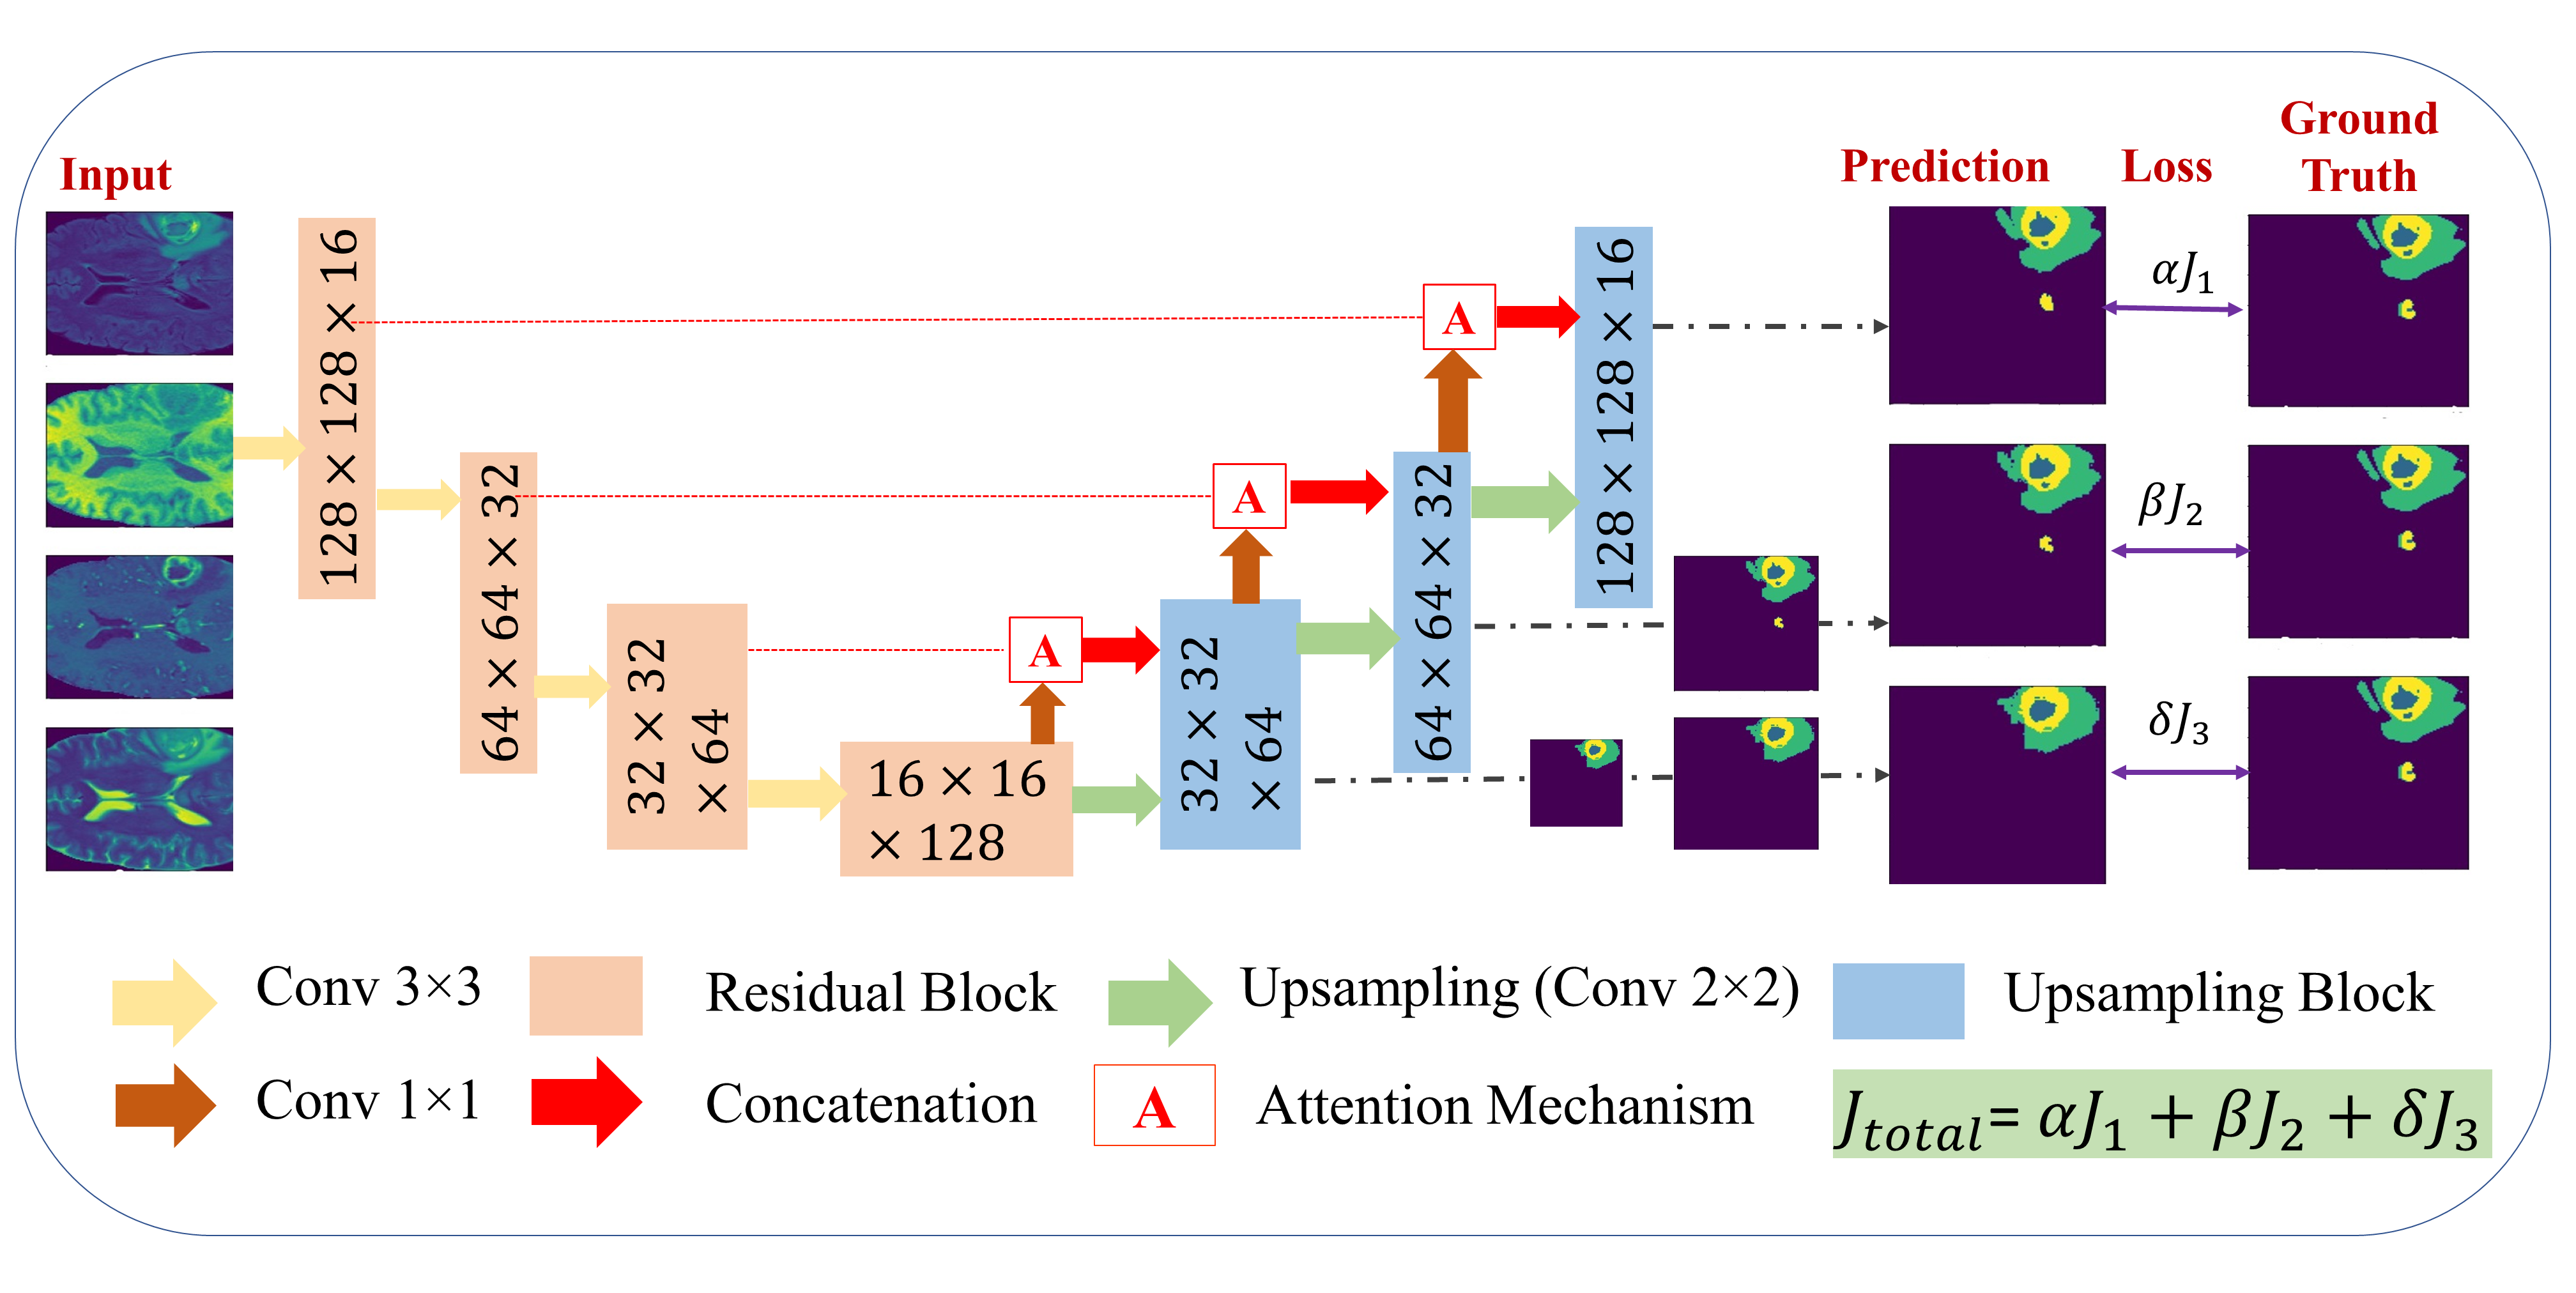
\includegraphics[width=1\linewidth]{model.png}
\caption{\justifying End-to-end network architecture of the proposed ARLU-Net. Implementation of loss function at each layer where $\alpha, \beta$, and $\delta$ parameters are defined to define participation of a layer loss value to total loss.}
\end{figure}
\end{frame}

\begin{frame}{Proposed attention mechanism}
\vspace{-4mm}
\begin{figure}[H]
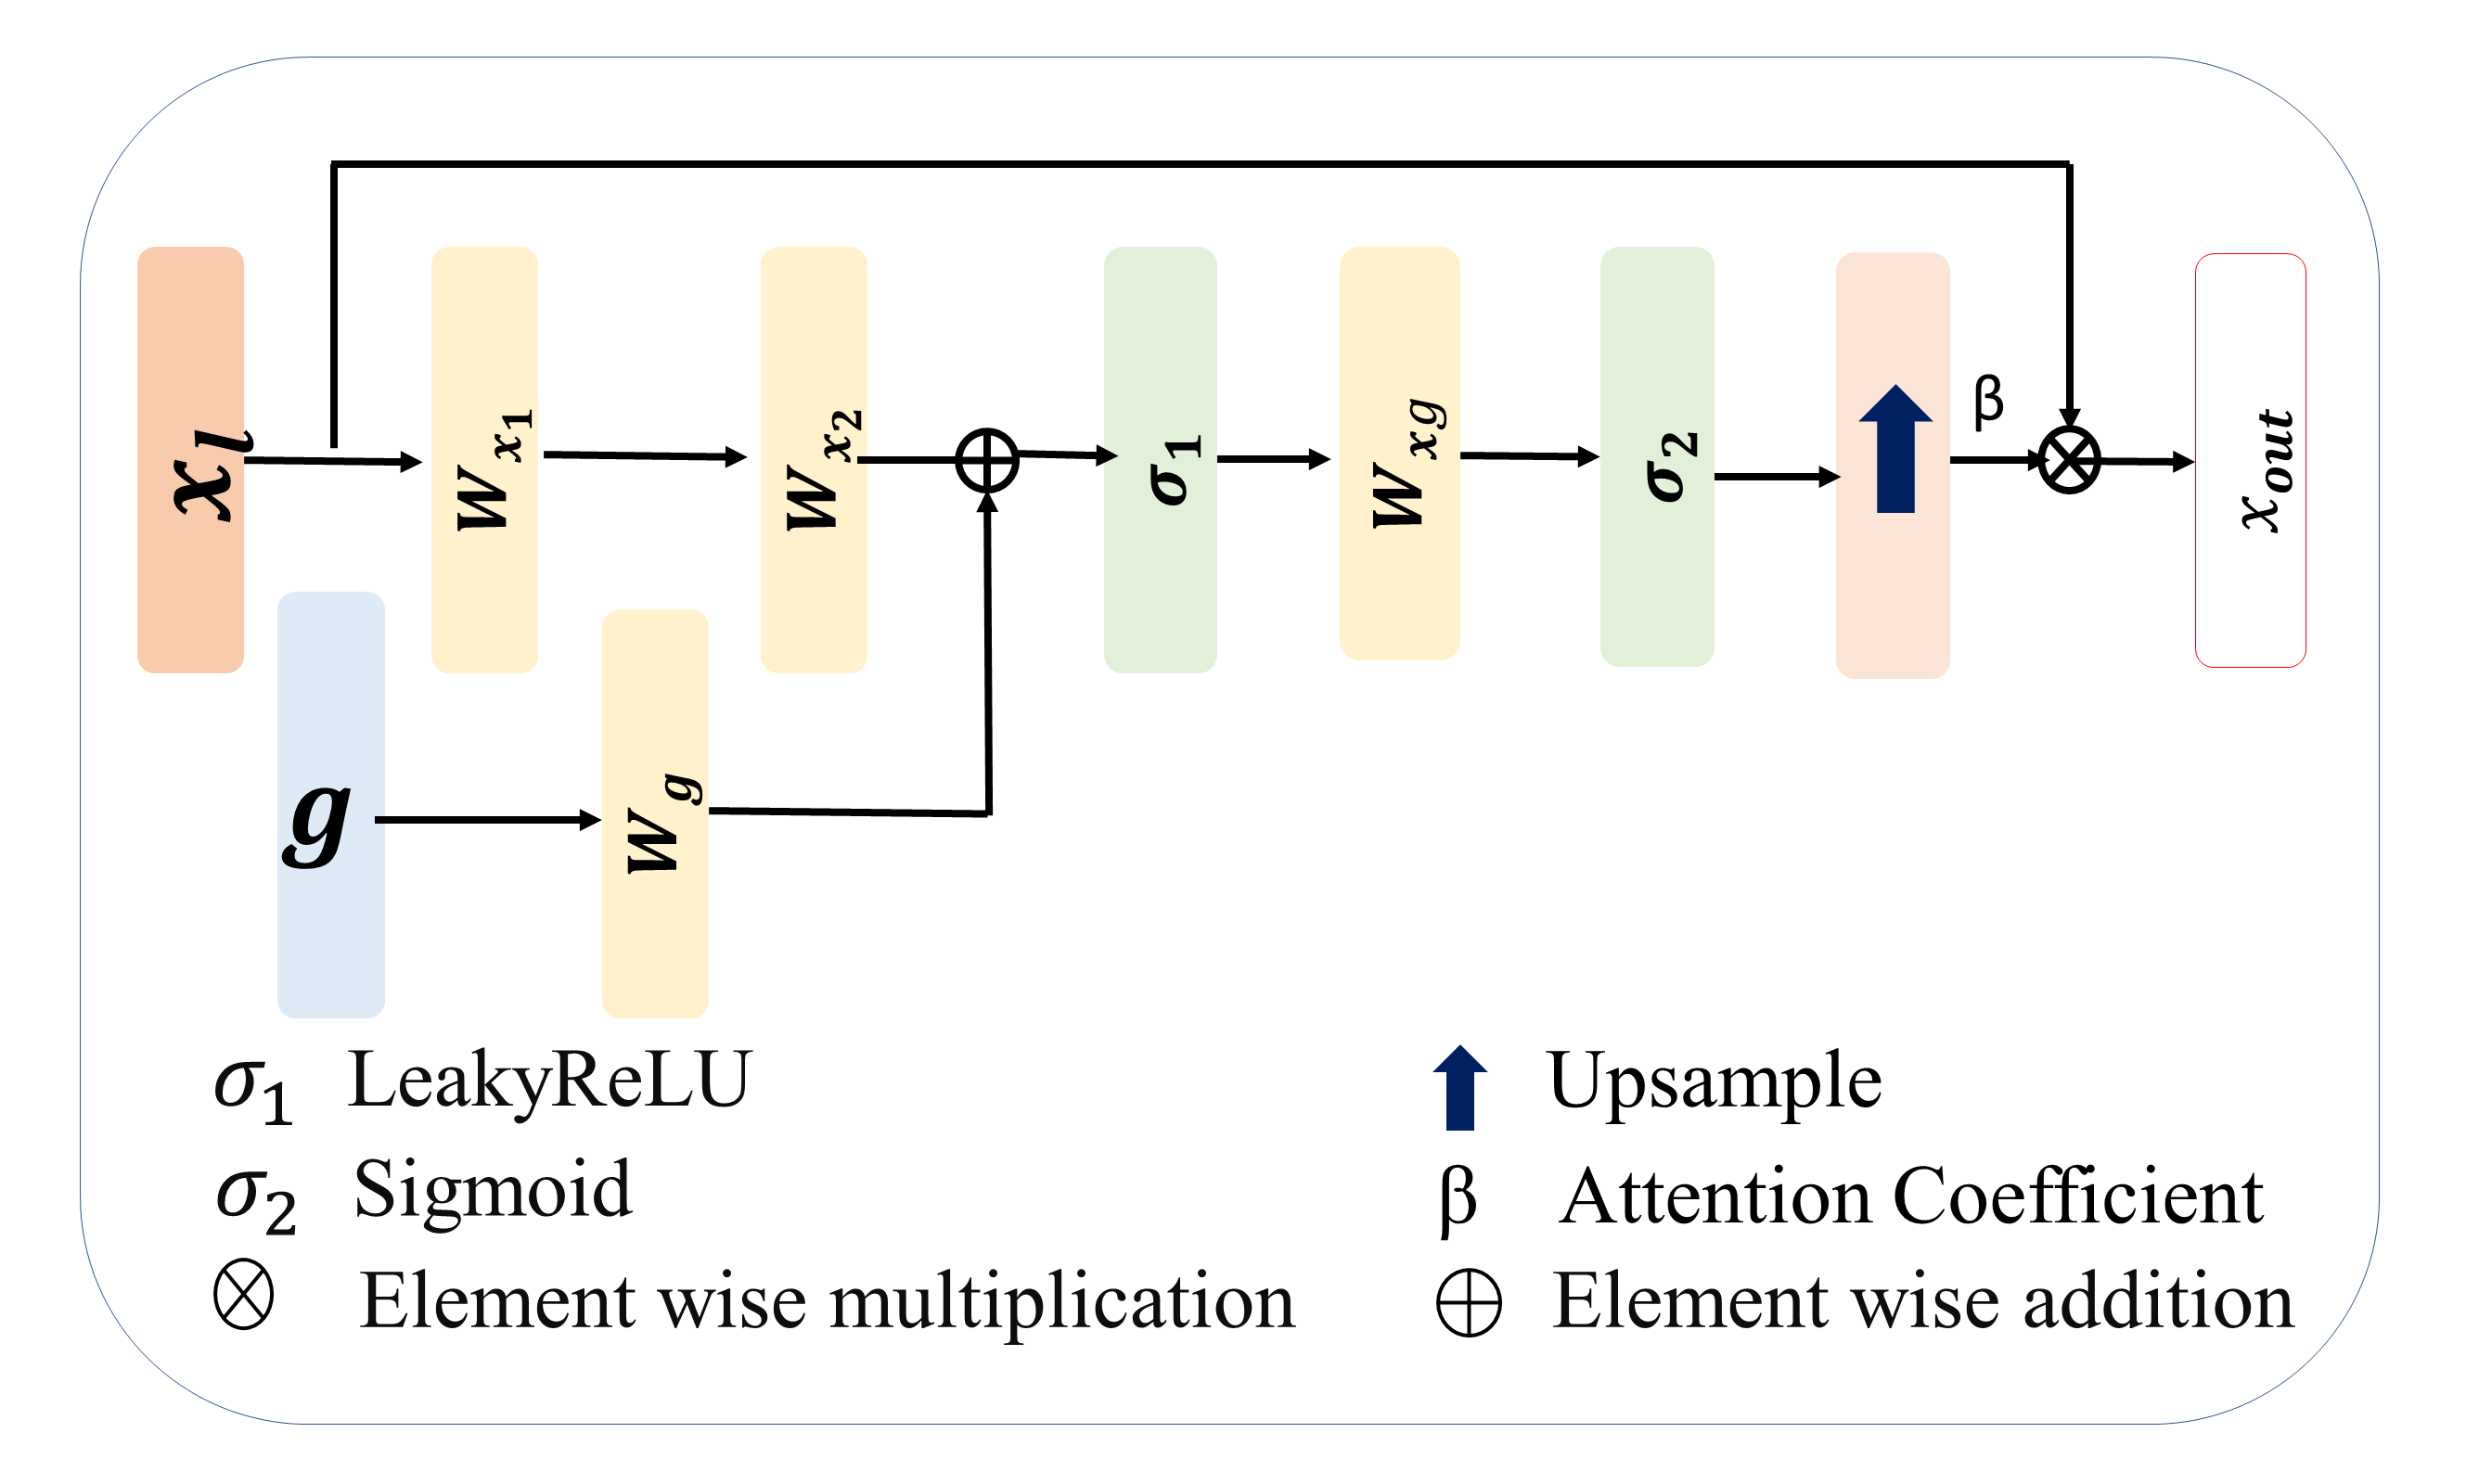
\includegraphics[width=0.7\linewidth]{attenton1.png}
\caption{\justifying The schematic diagram of attention gate where $x_l$ and $g$ are feature vector from layer $l$ and gating signal vectors from next lowest layer, respectively. $W_{x_1}$, $W_{x_2}$, $W_g$ and $W_{xg}$ are linear transformation. The output of the attention gate $x_{out}$ is element wise multiplication between $x_l$ and $\beta$ where $\beta$ is attention coefficient.}
\end{figure}
\vspace{-5mm}
\begin{equation}
\beta = \sigma_2(W_{xg} \ast (\sigma_1(W_{x_2} \ast (W_{x_1} \ast x) + W_g \ast g + b_1)) + b_2)
\label{eq2}
\end{equation}
\begin{equation}
x_{out} = x_l \cdot \beta
\end{equation}
\end{frame}

\section{Experimental results}
\begin{frame}{Experimental setup}
\vspace*{\fill}
    \begin{enumerate}
    \justifying
        \item We collected a dataset of 1251 patients from RSNA-ASNR-MICCAI Brain Tumor Segmentation (BraTS) Challenge 2021.
        \item We are using only 25 slices among 155 images of each patient because the remaining are noisy data.
        \item We use training, validation, and testing 23775, 5000, and 2500 in our proposed experimental analysis.
        \item Batch Size = $75$
        \item Learning Rate = 0.0001
        \item Evaluated our proposed model based on IoU and Dice Score.
   \end{enumerate}
    \vspace*{\fill}
\end{frame}

\begin{frame}{Experimental setup}
\vspace*{\fill}
\begin{table}[]
\caption{Information regarding WT, TC and ET}
\setlength{\tabcolsep}{2pt}
\begin{tabular}{|l|l|l|}
\hline
Brain tumor region & Types & Class label \\
    \hline
    Whole Tumor (WT) & Necrosis, Edema, Enhancing Tumor & 1,2,3\\
    \hline
    Tumor Core (TC) & Necrosis, Enhancing Tumor & 1,3\\
    \hline
    Enhancing Tumor (ET) & Enhancing Tumor & 3\\
    \hline        
\end{tabular}
\label{tab1}
\end{table}
\vspace*{\fill}
\end{frame}

\begin{frame}{Proposed loss function}

Weighted Dice Loss,
\begin{equation}
J_{WDL} = 1 - 2 \times \frac{\sum_{i}^{n}w_i \sum_{k}g_{ik} p_{ik}}{\sum_{i}^{n}w_i \sum_{k}(g_{ik}+p_{ik})}
\end{equation}
Weighted Focal Loss,
\begin{equation}
J_{WFL} = -\sum_{k}\sum_{i}^{n}w_i g_{ik} (1-p_{ik})^\gamma \log(p_{ik})
\label{eq8}
\end{equation}
where $n$ represent total number of labels, $w_i$ denotes weight assigned to $i^{th}$ label, $\gamma$ is hyperparameter for focal loss. $p_{ik}$ and $g_{ik}$ represent ($i^{th}$,$k^{th}$) pixel value of segmented image and ground truth image, respectively.
\end{frame}

\begin{frame}{Proposed loss function}
Combined loss function,
\begin{equation}
J_{Loss} = J_{WDL} + J_{WFL}
\end{equation}
Total loss of proposed network,
    \begin{equation}
            J_{total} = \alpha \times J_1 + \beta \times J_2 + \delta \times J_3
    \end{equation}
where $\alpha$, $\beta$ and $\delta$ are weights defined for $1^{st}$, $2^{nd}$, and $3^{rd}$ layer guided loss, respectively. Weights are defined according to priority as the 3rd layer is the final output that is given more priority than the other two layers. So from experiments, we selected $\alpha$ = $\beta$ = $0.125$ and $\delta$ = $0.5$.
\end{frame}

\begin{frame}{Evaluation metrics}
\vspace*{\fill}
    Dice Score,
    \begin{equation}
        DS_n = \frac{2 \times \sum_{}p_n\cdot g_n}{\sum_{}p_n + \sum_{}g_n}
    \end{equation}
Mean IoU,
    \begin{equation}
        IoU_n = \frac{\sum_{}p_n g_n}{\sum_{}p_n + \sum_{}g_n - \sum_{}p_n g_n}
    \end{equation}
    where $p_n$ and $g_n$ are predicted and ground truth  vectors for $n^{th}$ region respectively. A region in our brain tumor segmentation problem can be whole tumor, tumor core, and enhancing tumor.  
    \vspace*{\fill}
\end{frame}

\begin{frame}{Experimental result}
\vspace*{\fill}
    \begin{table}[H]
\centering
\caption{Segmentation result between the proposed model and state-of-art model based on BraTS-2021 dataset}
\begin{tabular}{ |p{2.5cm}|p{1cm}|p{1cm}|p{1cm}|p{1cm}|p{1cm}|p{1cm}|  }
\hline
Methods & \multicolumn{3}{c|}{\textbf{Mean IoU}} & \multicolumn{3}{c|}{\textbf{Dice Score}} \\
\cline{2-7}
  & WT & TC & ET & WT & TC & ET\\
\hline
\hline
U-Net \cite{10.1007/978-3-319-24574-4_28} & 0.7729 & 0.8569 & 0.8050 & 0.8719 & 0.9229 & 0.8919\\
\hline
V-Net \cite{Milletari2016VNetFC} & 0.8691 & 0.8533 & 0.8202 & 0.9300 & 0.9209 & 0.9012\\
\hline
ResU-Net \cite{SHEHAB2021404}& 0.8826 & 0.8845 & 0.8151 & 0.9376 & 0.9387 & 0.8982\\
\hline
ARU-Net\cite{MAJI2022103077} & \textcolor{red}{0.8895} & 0.8845 & 0.8381 & \textcolor{red}{0.9415} & 0.9387 & 0.9119\\
\hline
ARLU-Net & 0.8842 & \textcolor{red}{0.8877} & \textcolor{red}{0.8420} & 0.9385 & \textcolor{red}{0.9405} & \textcolor{red}{0.9142}\\
\hline
\end{tabular}
\end{table}
\vspace*{\fill}
\end{frame}

\begin{frame}{Experimental result}
\vspace*{\fill}
\begin{table}[H]
    \centering
    \caption{Comparison of proposed ARLU-Net model and the state-of-art model ARU-Net on BraTS 2021 dataset}
\begin{tabular}{ |p{2cm}|p{1.2cm}|p{1cm}|p{1cm}|p{1.2cm}|p{1cm}|p{1cm}|  }
\hline
Method & \multicolumn{3}{|c|}{Mean IoU} & \multicolumn{3}{|c|}{Dice Score} \\
\cline{2-7}
  & WT & TC & ET & WT & TC & ET\\
\hline
\hline
ARU-Net & 0.8895 & 0.8845 & 0.8381 & 0.9415 & 0.9387 & 0.9119\\
\hline
ARLU-Net & 0.8842 & 0.8877 & 0.8420 & 0.9385 & 0.9405 & 0.9142\\
\hline
Average Improvement & -0.0053 & \textcolor{red}{0.0032} & \textcolor{red}{0.0039} & -0.0030 & \textcolor{red}{0.0018} & \textcolor{red}{0.0023}\\
\hline
\end{tabular}
\end{table}
\vspace*{\fill}
\end{frame}


\begin{frame}{Experimental result}
\vspace*{\fill}
\begin{table}
\centering
\caption{Comparison of state-of-art model with ARLU-Net model based on total number of trainable parameters defined for a network.}
\label{table}
\setlength{\tabcolsep}{3pt}
\begin{tabular}{|l|l|l| }
\hline
\textbf{Methods} & \textbf{Total parameters} & \textbf{Comparison with ARLU-Net}\\
\hline
\hline
ARLU-Net & \textcolor{red}{527,631 = p} & $p$\\
\hline
U-Net & 1,941,300 & 3.6 $\times$ $p$  \\
\hline
V-Net & 2,273,284 &  4.3 $\times$ $p$\\
\hline
ResU-Net & 9,081,348 &  17.2 $\times$ $p$\\
\hline
ARU-Net & 2,159,100 &  4.1 $\times$ $p$\\
\hline
\end{tabular}
\end{table}
\vspace*{\fill}
\end{frame}



\begin{frame}{Experimental result}
\vspace*{\fill}
    \begin{table}
\caption{Comparison of ARLU-Net model on basis of different combination of loss function.}
\label{table}
\setlength{\tabcolsep}{3pt}
\begin{tabular}{|l|l|l|}
\hline
\textbf{Combined Loss Function} & \textbf{Average Mean IoU} & \textbf{Average Dice Score} \\
\hline
\hline
 ARLU-Net (WDL) & 0.8697 & 0.9302\\
 \hline
 ARLU-Net (DL + FL) & 0.8652 & 0.9275\\
 \hline
 ARLU-Net (WDL + FL) & 0.8669 & 0.9286 \\
 \hline
 %ARLU-Net (WDL + WCL) & 0.8674 & 0.9289\\
 %\hline
 ARLU-Net (WDL + WFL) & \textcolor{red}{0.8713} & \textcolor{red}{0.9311}\\
\hline
\end{tabular}
\end{table}
\vspace*{\fill}
\end{frame}

\begin{frame}{Experimental result}
\vspace*{\fill}
    \begin{table}
\caption{Comparison of our proposed model ARLU-Net based on hyperparameter gamma defined within range, $\gamma \in [0,4]$ with weighted focal loss defined at \eqref{eq8}}
\label{table}
\setlength{\tabcolsep}{3pt}
\begin{tabular}{|l|l|l| }
\hline
\textbf{Hyperparameter $\gamma$} & \textbf{Average Mean IoU} & \textbf{Average Dice Score} \\
\hline
\hline
0 & 0.8674 & 0.9288\\
\hline
1 & 0.8659 & 0.9279\\
\hline
2 & \textcolor{red}{0.8713} & \textcolor{red}{0.9311}\\
\hline
3  & 0.8672 & 0.9287\\
\hline
4 & 0.8675 & 0.9289\\
\hline
\end{tabular}
\label{tab5}
\end{table}
\vspace*{\fill}
\end{frame}

\begin{frame}{Experimental result}
\vspace{-5mm}
    \begin{figure}[H]
        \centering
        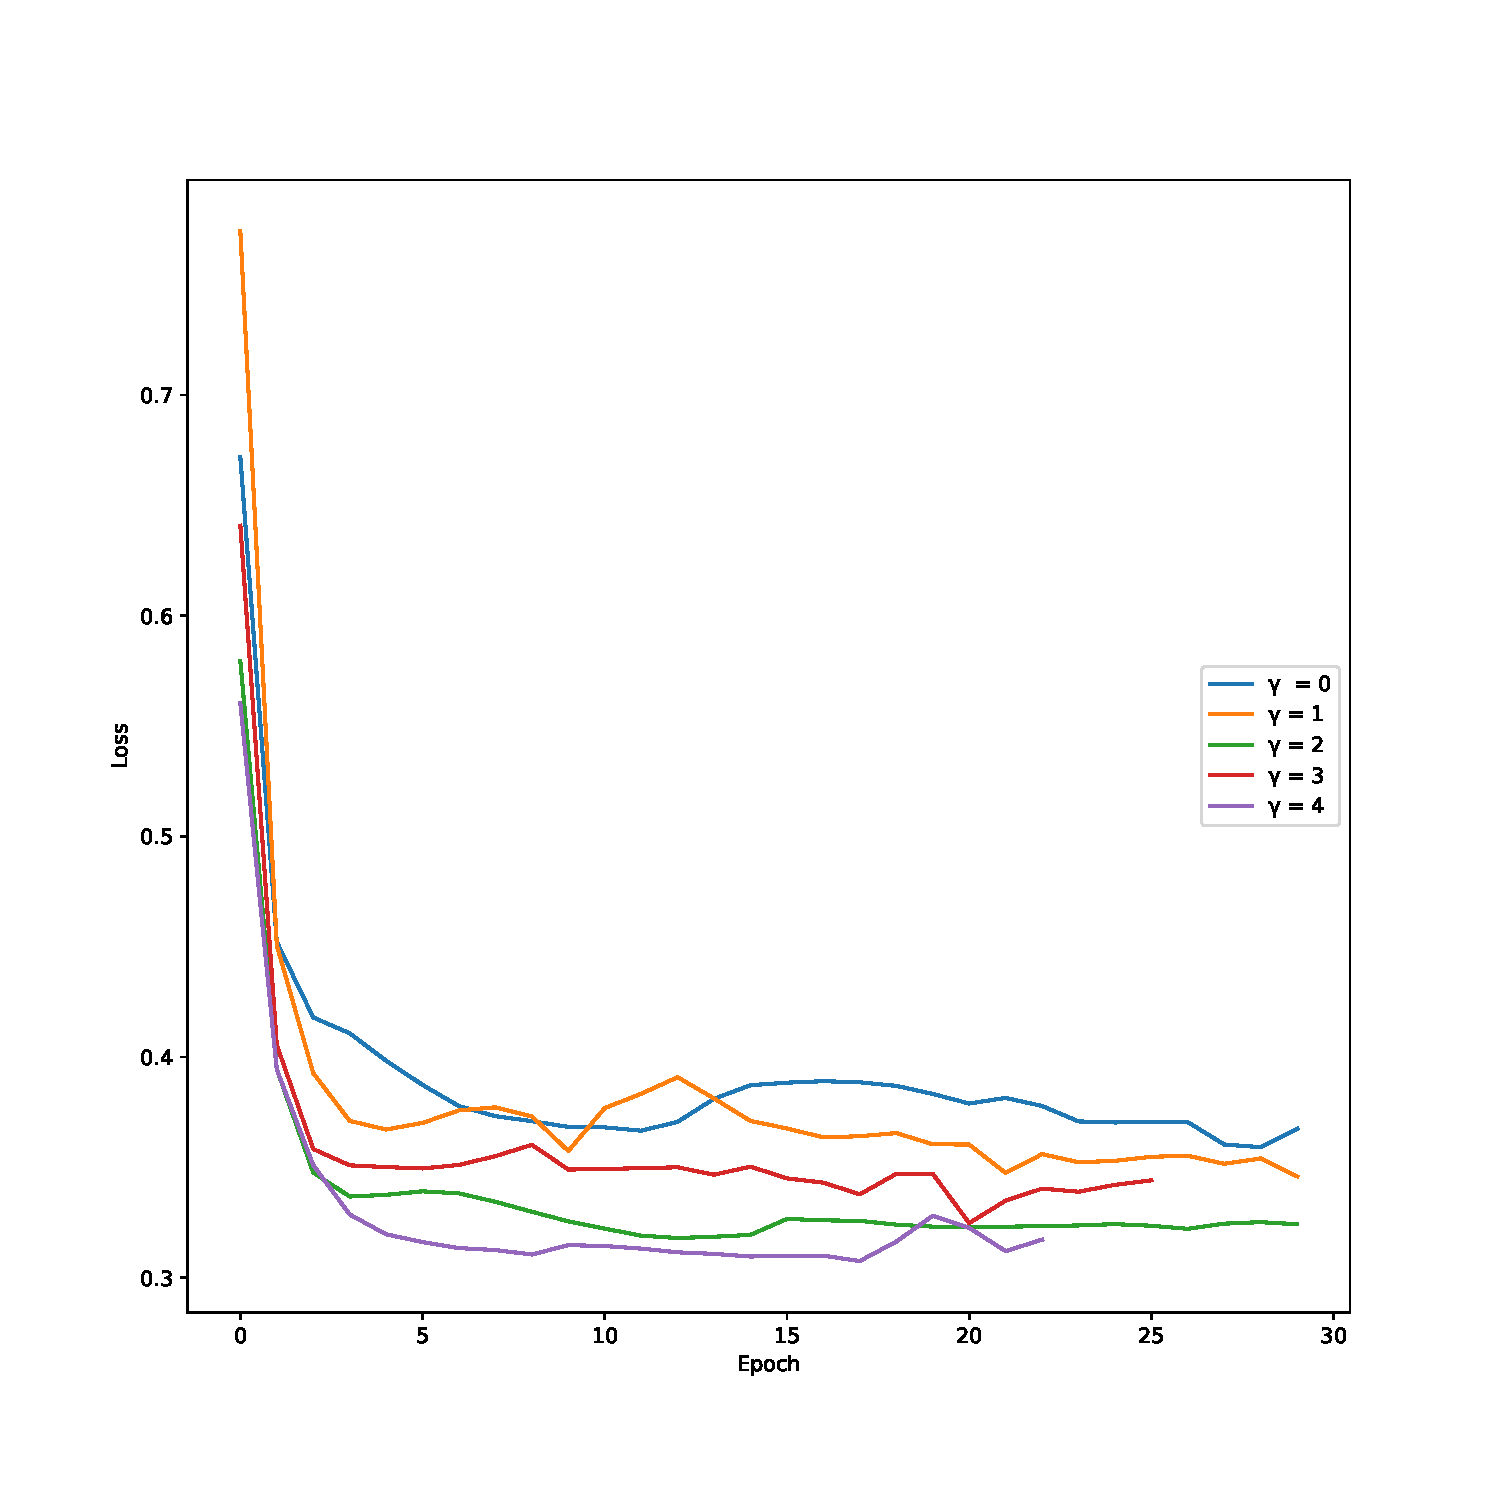
\includegraphics[width=10cm,height=6.9cm]{result.pdf}
        \centering
        \caption{Comparison of our proposed model ARLU-Net based on hyperparameter $\gamma$ defined with weighted focal loss in equation \eqref{eq8}}
    \end{figure}
\end{frame}

\begin{frame}{Segmented vs ground truth images on BraTS-2021 dataset}
\vspace{-1em}
\begin{figure}[H]
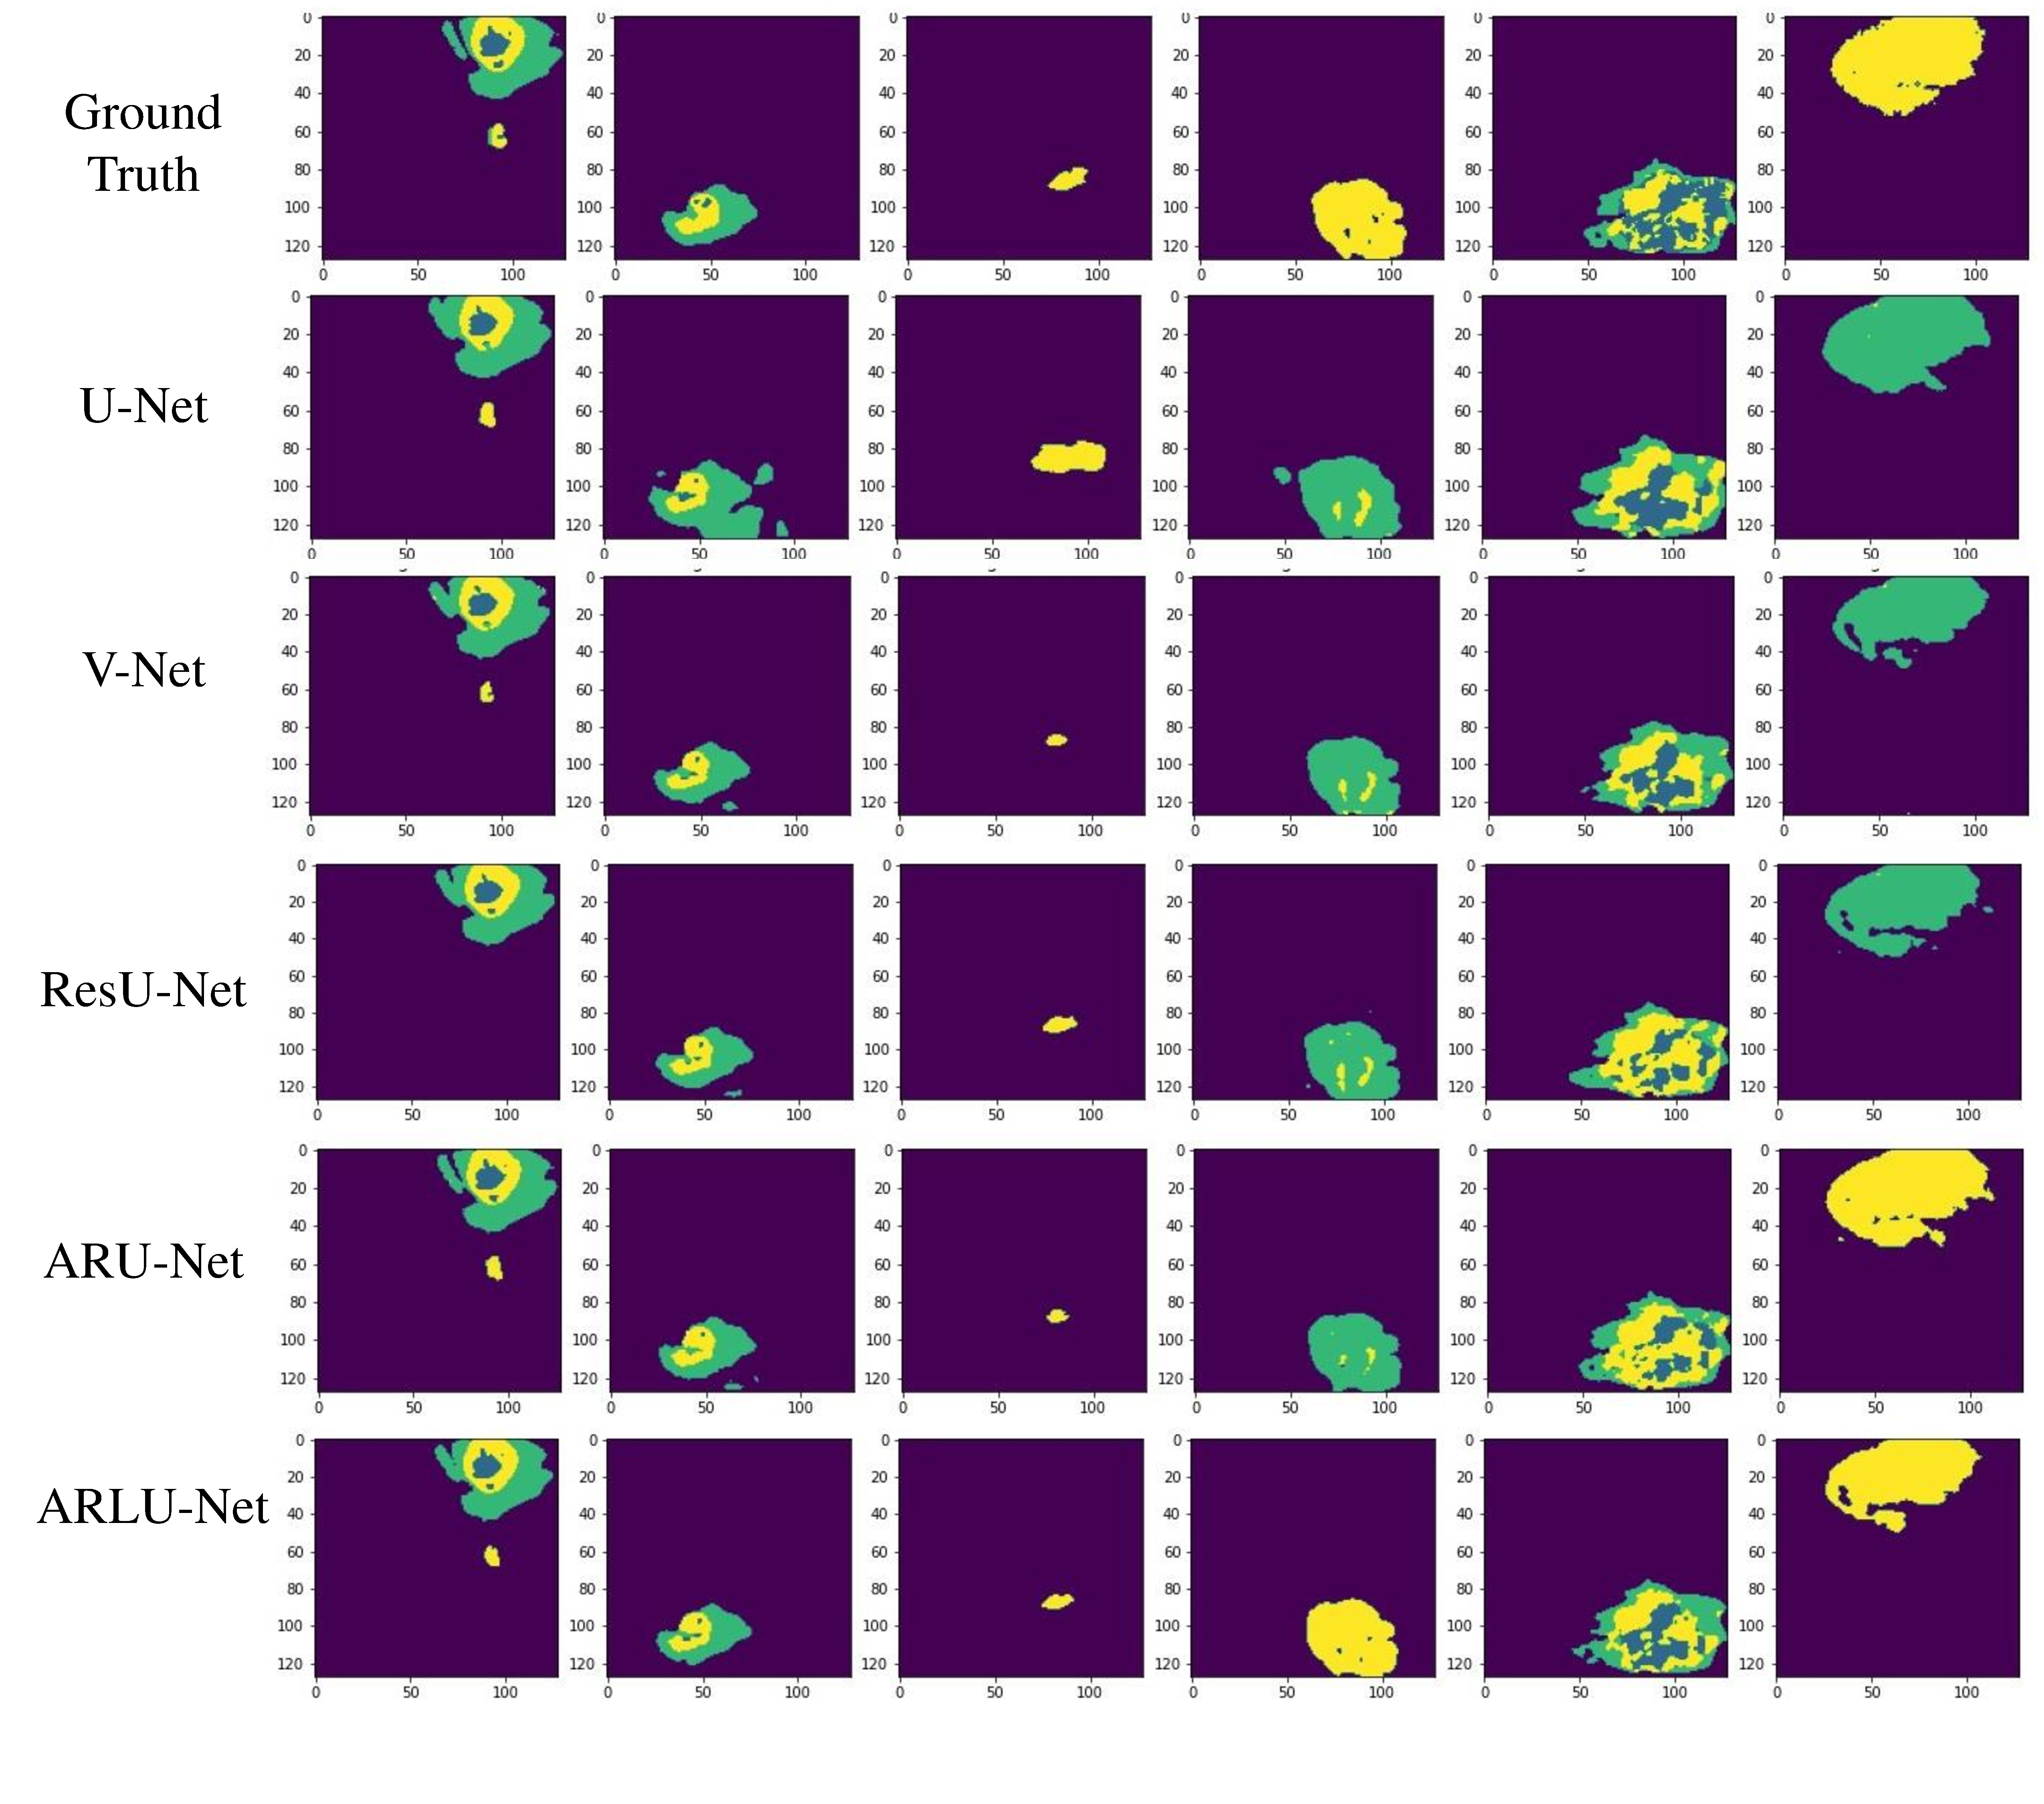
\includegraphics[width=0.8\linewidth,page=1]{segmentation.pdf}
\centering
\end{figure}
\end{frame}

\section{Conclusion}
\begin{frame}{Experimental conclusion}
\vspace*{\fill}
    \begin{enumerate}
    \justifying
        \item We proposed a light-weight deep learning model, \emph{i.e.,} Attention-based Residual Light U-Net, which efficiently explores the attention gate for semantic segmentation of Brain Tumor.
        \item Dataset plays a vital role in our research because we perform on 31,275 samples, which is comparatively more than previously used.
        \item The hypothetical dilemma considered for ARLU-Net has achieved a better result by adding $1 \times 1$ convolution to the attention gate. So here is the question if we add more $1 \times 1$ convolution to the attention gate, our model will get trained to a specific tumor region instead of other regions.
        \item Brain tumor segmentation is still a challenging task due to limited patient samples and significant variation in tumor size in MRI brain images. 
        \item It also has limitations in working with 2D models using 3D MRI images.
    \end{enumerate}
    \vspace*{\fill}
\end{frame}

\section{Future work}
\begin{frame}{Future work}
\vspace*{\fill}
\begin{enumerate}
    \item Future, we will be working on 3D model architecture instead of 2D to improve segmentation performance and working on large samples of patients.
    \item After implementing the model, we will present in brain tumor segmentation challenge to compete against the temporary work in the field.
\end{enumerate}
\vspace*{\fill}
\end{frame}
    
\begin{frame} [allowframebreaks]\frametitle{References}
    \tiny\bibliographystyle{ieeetr}
    \bibliography{ref_ppt}
    \nocite{*}
\end{frame}


\begin{frame}[standout]
\vspace{35mm}
\centering \Huge
  \emph{Thank You}
\end{frame}
\end{document}